\problemname{Braille Addition}
To save on electricity bills, Lydia has decided to do math without lighting. Without lighting, it is
difficult to distinguish regular text, so Lydia plans to switch to Braille. In Braille, each character
is written as a grid of $3 \times 2$ dots, where some are raised. In Figure~\ref{fig:braille}, you can
see how the ten digits are written in Braille.

\begin{figure}[h]
    \centering
    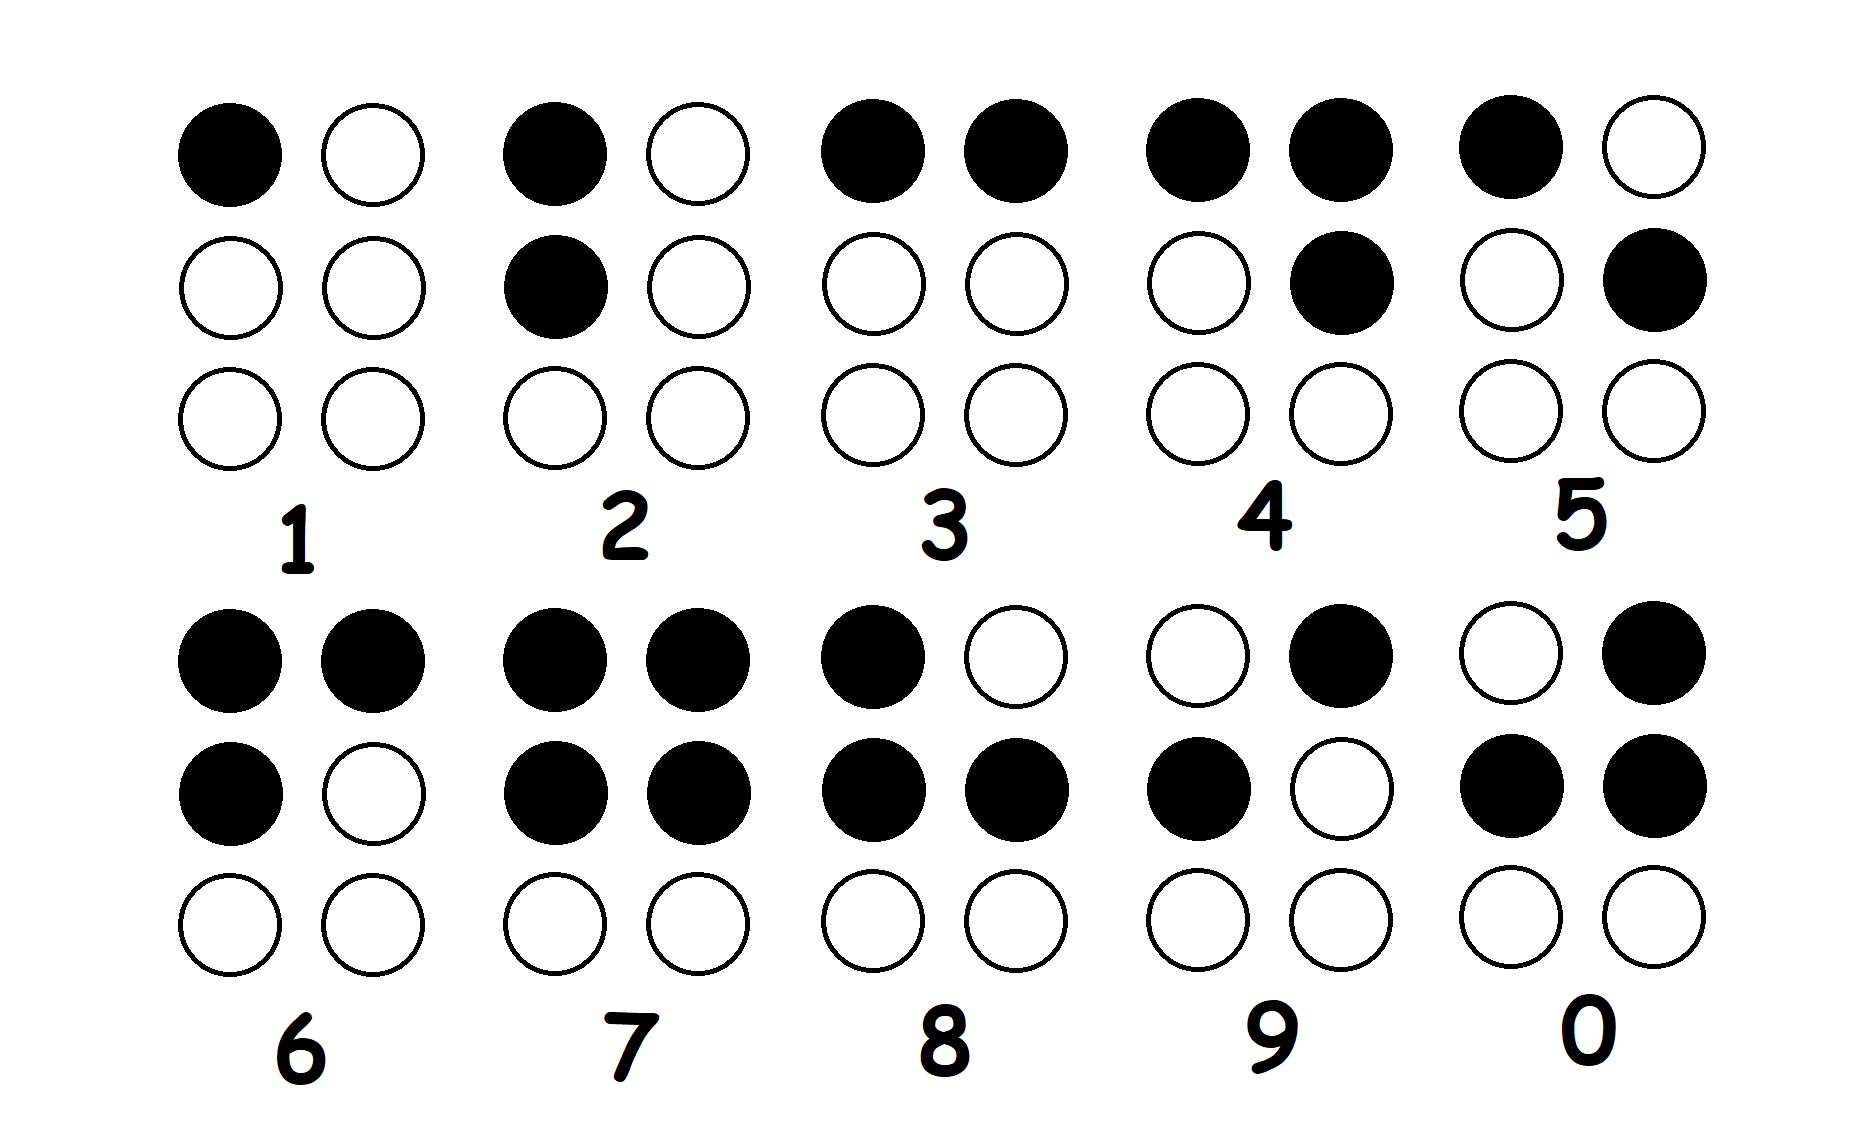
\includegraphics[width=0.75\textwidth]{braille.png}
    \caption{The Braille digits 0 to 9. The raised dots are indicated by a filled circle.}
    \label{fig:braille}
\end{figure}

She now needs your help to verify her calculations. Write a program that finds the sum of two numbers in Braille form.

\section*{Input}
The first line contains an integer $N$ ($1 \leq N \leq 9$), the number of digits in the first number.

The following three lines contain $N$ Braille digits representing the first number.

The next line contains an integer $M$ ($1 \leq M \leq 9$), the number of digits in the second number.

The following three lines contain $M$ Braille digits representing the second number.

The Braille digits are given as a matrix of $3 \times 2$ characters, where an asterisk ('\texttt{*}') indicates a raised dot and a period ('\texttt{.}') indicates a dot that is not raised.

The digits are given in the same order as a regular decimal number, so that the last digit corresponds to the unit digit of the number. The numbers have no leading zeros, except in the case the number is $0$.

\section*{Output}
Print sum of the two numbers in braille.

\section*{Points}
Your solution will be tested on several test case groups.
To get the points for a group, it must pass all the test cases in the group.

\noindent
\begin{tabular}{| l | l | p{12cm} |}
  \hline
  \textbf{Group} & \textbf{Point value} & \textbf{Constraints} \\ \hline
  $1$    & $31$      & Only the braille digit $1$ appears in the input. \\ \hline
  $2$    & $69$      & No additional constraints. \\ \hline
\end{tabular}

\section*{Explanation of samples}
The first number consists of the Braille digits $1$, $6$, and $0$, which together form the number $160$.
The second number consists of the Braille digits $1$ and $6$, which together form the number $16$.
The sum is $160 + 16 = 176$.
